\documentclass[11pt,openany]{memoir}
\usepackage[usenames,dvipsnames]{xcolor}
\usepackage{amssymb}
\usepackage{amsmath}
\usepackage{amsthm}
\usepackage{url}
\usepackage{xspace}
\usepackage[margin=2.5cm]{geometry}
%\usepackage{tikz}
%\usetikzlibrary{positioning,calc,matrix,arrows}
%\usepackage{pgfplots}
\usepackage{listings}
\usepackage{color}
\usepackage{textcomp}
\usepackage{fancyvrb}
\usepackage{array}
\usepackage{dirtytalk}
\usepackage{graphicx}
\usepackage[colorlinks]{hyperref}
\usepackage{cleveref}

% NOTE: This template is based on the MatConvNet manual written by Andrea Vedaldi, Karel Lenc and Ankush Gupta.

\newtheorem{example}{Example}
\newtheorem{lemma}{Lemma}

\newcommand{\real}{\mathbb{R}}
\newcommand{\xx}{\mathbf{x}}
\newcommand{\yy}{\mathbf{y}}
\newcommand{\pp}{\mathbf{p}}
\newcommand{\hh}{\mathbf{h}}
\newcommand{\diag}{\operatorname{diag}}
\newcommand{\bone}{\mathbf{1}}
\newcommand{\FF}{\mathcal{F}}
\newcommand{\ththeta}{\pmb{\theta}}
\newcommand{\EE}{\mathbb{E}}
\DeclareMathOperator{\dd}{\text{d}}
\newcommand{\vv}{\operatorname{vec}}
\newcommand{\tr}{\operatorname{tr}}
%\newcommand{\by}{\mathbf{y}}
%\newcommand{\bc}{\mathbf{c}}
%\newcommand{\bz}{\mathbf{z}}
%\newcommand{\bff}{\mathbf{f}}
%\newcommand{\bg}{\mathbf{g}}
%\newcommand{\br}{\mathbf{r}}
%\newcommand{\bw}{\mathbf{w}}
%\newcommand{\bp}{\mathbf{p}}
%\newcommand{\bfs}{\mathbf{s}}
%\newcommand{\bfe}{\mathbf{e}}
%\newcommand{\samsays}[1]{\textcolor{RubineRed}{[S: #1]}}

%\newcommand{\argmin}{\operatornamewithlimits{argmin}}
%\newcommand{\argmax}{\operatornamewithlimits{argmax}}
%\newcommand{\sign}{\operatornamewithlimits{sign}}
%
%\tikzstyle{block} = [draw, rectangle, minimum height=3em, minimum width=3em]
%\tikzstyle{data} = []
%\tikzstyle{datac} = [draw, circle, minimum height=2.5em, minimum width=2.5em,inner sep=3pt,font=\footnotesize]
%\tikzstyle{par} = [draw, circle, minimum height=2.5em, minimum width=2.5em,fill=black!20,inner sep=3pt,font=\footnotesize]
%\tikzstyle{pinstyle} = [pin edge={to-,thin,black}]
%\tikzstyle{to} = [->,>=stealth',shorten >=1pt,semithick]
%\tikzstyle{from} = [<-,>=stealth',shorten >=1pt,semithick]
%\tikzstyle{bp} = [draw=blue,text=blue]
%\tikzstyle{bpl} = [draw=blue!40]
%\tikzstyle{bpe} = [text=blue,draw=none]

\VerbatimFootnotes

\setsecnumdepth{subsection}
\settocdepth{subsection}

\definecolor{listinggray}{gray}{0.9}
\definecolor{lbcolor}{rgb}{0.8,0.8,0.8}
\lstset{
	%backgroundcolor=\color{lbcolor},
	tabsize=4,
	%rulecolor=,
	language=matlab,
	basicstyle=\small,
	%upquote=true,
	%columns=fullflexible,
	%showstringspaces=false,
	extendedchars=true,
	%breaklines=false,
	%prebreak = \raisebox{0ex}[0ex][0ex]{\ensuremath{\hookleftarrow}},
	%frame=single,
	%showtabs=false,
	%showspaces=false,
	%showstringspaces=false,
	%identifierstyle=\ttfamily,
	keywordstyle=\color[rgb]{0,0,1},
	commentstyle=\itshape\color[rgb]{0.133,0.545,0.133},
	stringstyle=\color[rgb]{0.627,0.126,0.941},
}
%\lstMakeShortInline[columns=fullflexible, breaklines = true,
% breakatwhitespace = true]!

\title{Optimization for Applied Computer Vision}
\author{
Samuel Albanie
}
\date{}

% REMOVE TO FIX COMPILATION
\hypersetup{
  pdfinfo={
    Title={Optimization for Applied Computer Vision},
    Author={Samuel Albanie},
        Subject={Notes on Mathematics},
    Keywords={computer vision, differentials, machine learning}
  }
}

\sloppy

% ------------------------------------------------------------------
\begin{document}
% ------------------------------------------------------------------

%\end{document}

\frontmatter
\maketitle{}

\begin{abstract}
The aim of this note is to aggregate some useful information relating to optimization in computer vision research.
The goal is to develop it over time and therefore it should be considered a work-in-progress.  Consequently any contributions, feedback or notifications of mistakes are much appreciated\footnote{Feel free to contact me by raising an issue on the github page, submitting a pull request directly (\mbox{\url{https://github.com/albanie/derivations})}}).
\end{abstract}
\clearpage

\tableofcontents*
\clearpage

\mainmatter
\chapter{Introduction}\label{sec:intro}

Calculus plays a central role in computer vision. As the community has integrated ever more closely with techniques from machine learning, statistics and optimisation, the ability to differentiate vector and matrix functions has become more useful to computer vision researchers.  Unfortunately, multivariate calculus, when performed with indices over element locations is a fairly tricky business to build an intuition for.  Although the index-based approach has the majority of the market share in the research world, there is an alternative: the slightly lesser known method of \textit{matrix differentials}.  We have found this alternative approach to be significantly simpler, more intuitive and faster to work with.  

Finally, we note that the widespread adoption of automatic differentiation (autodiff) has been a major boon to the whole community, in many cases obviating the need to perform arduous pen and paper derivations.  The goal of these notes is not to encourage the reader to avoid using autodiff, but to assist them in understanding, on a mathematical level, what is going on \say{under the hood}.


\section{Useful Resources}

There are a number of extremely good references for getting to grips with the calculus of vector and matrix functions.  Below are a few that we have found particularly useful, providing much of the material for these notes:

\begin{itemize}
\item Written by econometricians Magnus and Neudecker (originally in $1988$, but revised several times), \textit{Matrix differential calculus with applications in statistics and econometrics} is the canonical reference for matrix differential calculus~\cite{magnus1988matrix}.
\item The fundamentals of working with matrices \cite{searle2017matrix}.
\item \cite{kinghorn1996integrals}, \cite{minka2000old} and \cite{petersen2008matrix} each contain a large number of highly useful results and are good as quick references.
\item The MatConvNet manual \cite{vedaldi2015matconvnetmanual} provides carefully worked through examples of matrix derivatives.  While the emphasis is primarily on index-based derivations, it provides the derivatives of many common neural network computation blocks in matrix form and is very useful as a reference. 
\end{itemize}
\chapter{Computational Complexity} \label{chap:computational-complexity}

The goal of optimization is to find the best solution to a problem.  However, in many practical cases, the quality of the solution may be a less important factor than the total resources that must be expended in finding the solution.   There is a large field of research which focuses on this issue of \textit{computational complexity}: how long will it take to solver a problem, or can the problem be solved at all?

One popular categorisation of optimisation/decision problems is linked to the concept of a Turing Machine (TM), depicted in Fig.~\ref{fig:TM}. This is a  construct introduced in a landmark paper by Alan Turing in the 1930s \cite{turing1937computable}, in which he provided a proof that certain decision problems are \textit{undecidable}.  A TM is a device with a read/write head which, at any point in time, points to a single location on a tape of symbols.  All symbols on the tape come from a finite alphabet $\Sigma_{\text{tape}}$ (in the figure, the alphabet contains three symbols, $\Sigma_{\text{tape}} = \{0, 1, b\}$, where $b$ is used to denote a blank space).  In addition to being able to read and write from the tape, the machine itself maintains a state, which consists of a symbol $s_i$ from a second finite alphabet, $\Sigma_{\text{machine}} = \{s_1, \dots, s_m\}$. Finally, it has access to a set of instructions which take the form: \textit{if the tape symbol is $t_i$ and the state symbol is $s_i$, then write symbol $t_j$ to the current position, change state to $s_j$ and move one step in direction $D$}.  Here the direction can be L (left) or R (right).  An instruction can be therefore written as a $5$-tuple $(t_i, s_i, t_j, s_j, D)$.  The machine continues to run until it reaches a predefined \textit{accepting state}. There is a full worked example of writing a program that leads to a Turing machine copying an input sequence in \cite{turingMachines}.



\begin{figure}
\centering
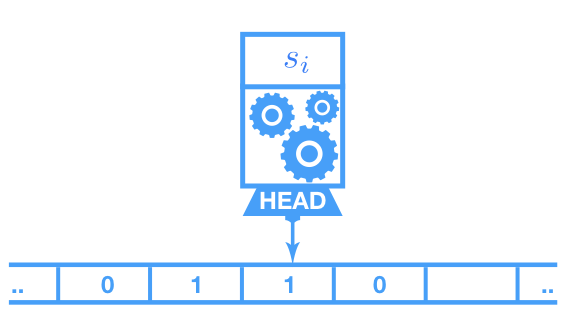
\includegraphics[width=0.5\textwidth]{figs/turing-machine-fig-001.png}
\caption{The Turing machine: a simple device with a read/write head which points to a single cell location on a tape of symbols.  The machine maintains a single state (currently $s_i$). \label{fig:TM}}	
\end{figure}

For the purposes of analysing the complexity of a program, we can define two distinct types of Turing machine. The first is the \textit{deterministic} Turing machine (DTM).  For any given machine state and tape symbol pairing, the instructions for the DTM can prescribe at most one action. The second type of machine is the \textit{non-deterministic} Turing machine (NTM), which allows instructions to specify multiple actions as outcomes for a given input configuration.  Both machines have the same \say{power}, in the sense that they can both solve the same types of problems.  However, the speed at which they can solve them can differ dramatically.  At each instruction with multiple outcomes, the NTM can branch (we can think of the machine as cloning itself and sending one clone along each output action), enabling it to explore an exponentially large space of execution paths.  By contrast, the DTM may only proceed along a single execution path at a time.  These concepts are useful because they provide a way to describe which problems are \say{exponentially expensive}.

Specifically, we define the class of decision problems \textit{P}, as those that can be solved by a DTM in polynomial time (by which we mean that the time is a polynomial function of the input).  We further define the class \textit{NP}, as those that can be solved by an NTM in polynomial time (the \say{N} here stands for non-deterministic). It is also popular to use the equivalent definition of NP as the set of problems that can be \textit{verified} in polynomial time by a DTM (intuitively, we can imagine following just the branch taken by the NTM clone that eventually reaches the accepting state with a single DTM).  The question of whether these two problem classes are equivalent is considered one of the classic (unsolved) problems of computer science \cite{pvnp}.

There are two further categories which are often used to describe problem complexities. A problem $t$ is said to be \textit{NP-hard} if it satisfies the property that any problem in NP can be reduced to problem $t$ in \textit{polynomial time} by a DTN.  A problem is said to be \textit{NP-complete} if, in addition to being NP-hard, it also lies in NP.  
\chapter{Multi-objective Optimization} \label{chap:multi-objective}

% ------------------------------------------------------------------
\bibliographystyle{plain}
\bibliography{../bib/refs.bib}
\end{document}
% ------------------------------------------------------------------

